\documentclass[tikz, border=10pt]{standalone}

\usepackage{tikz}
\usetikzlibrary{shapes.geometric, arrows.meta, positioning, fit, backgrounds}

% Color palette
\definecolor{boxblue}{RGB}{70, 130, 180}
\definecolor{boxgreen}{RGB}{60, 160, 100}
\definecolor{boxorange}{RGB}{210, 120, 50}
\definecolor{boxgray}{RGB}{100, 100, 110}
\definecolor{lightblue}{RGB}{220, 235, 250}
\definecolor{lightgreen}{RGB}{220, 245, 230}
\definecolor{lightorange}{RGB}{250, 235, 215}
\definecolor{lightgray}{RGB}{240, 240, 245}

\tikzset{
  mainbox/.style={
    rectangle, rounded corners=4pt,
    minimum width=5cm, minimum height=0.9cm,
    draw=#1!80!black, fill=#1!15,
    font=\small\bfseries, text centered
  },
  contentbox/.style={
    rectangle, rounded corners=3pt,
    minimum width=1.6cm, minimum height=0.75cm,
    draw=#1!80!black, fill=#1!15,
    font=\scriptsize, text centered
  },
  arrow/.style={
    -Stealth, thick, color=boxgray
  },
  groupbox/.style={
    rectangle, rounded corners=6pt,
    draw=boxgray!60, dashed, fill=lightgray,
    inner sep=8pt
  }
}

\begin{document}
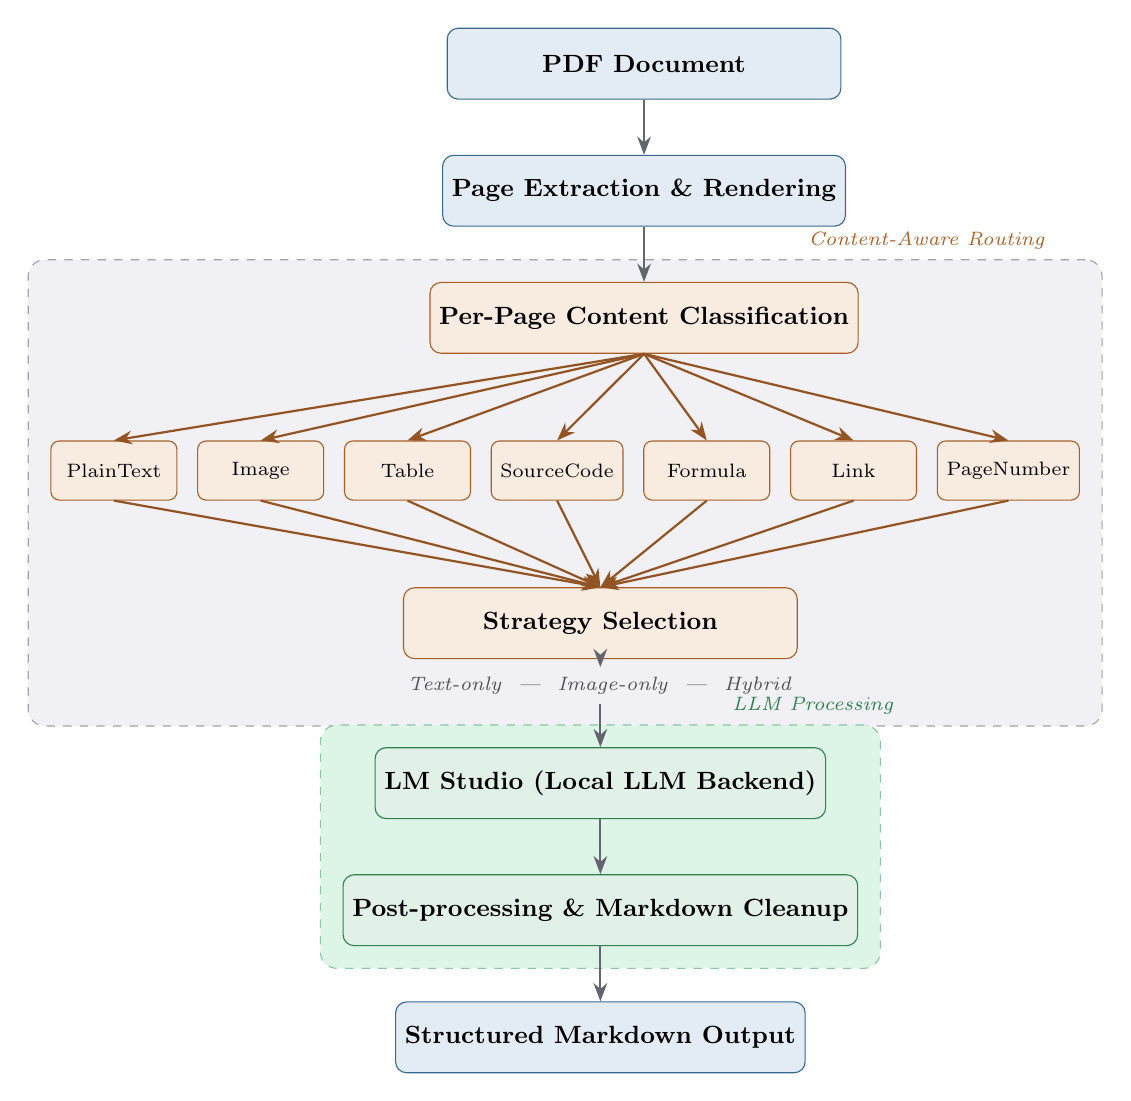
\begin{tikzpicture}[node distance=0.7cm and 0.4cm]

  % ── Input ──────────────────────────────────────────────
  \node[mainbox=boxblue] (pdf) {PDF Document};

  % ── Page extraction ────────────────────────────────────
  \node[mainbox=boxblue, below=of pdf] (extract)
    {Page Extraction \& Rendering};

  % ── Content classifier ─────────────────────────────────
  \node[mainbox=boxorange, below=of extract] (classify)
    {Per-Page Content Classification};

  % ── Content type nodes (row) ───────────────────────────
  \node[contentbox=boxorange, below left=1.1cm and 3.2cm of classify]
    (ctext)   {Plain\\Text};
  \node[contentbox=boxorange, right=0.25cm of ctext]
    (cimage)  {Image};
  \node[contentbox=boxorange, right=0.25cm of cimage]
    (ctable)  {Table};
  \node[contentbox=boxorange, right=0.25cm of ctable]
    (ccode)   {Source\\Code};
  \node[contentbox=boxorange, right=0.25cm of ccode]
    (cformula){Formula};
  \node[contentbox=boxorange, right=0.25cm of cformula]
    (clink)   {Link};
  \node[contentbox=boxorange, right=0.25cm of clink]
    (cpageno) {Page\\Number};

  % ── Strategy selector ──────────────────────────────────
  \node[mainbox=boxorange,
        below=1.1cm of ctable,
        xshift=2.45cm]
    (strategy) {Strategy Selection};

  % ── Strategy sub-labels ────────────────────────────────
  \node[font=\scriptsize, below=0.1cm of strategy,
        text=boxgray!80!black]
    (strats) {\textit{Text-only \ | \ Image-only \ | \ Hybrid}};

  % ── LM Studio ─────────────────────────────────────────
  \node[mainbox=boxgreen, below=0.55cm of strats] (lm)
    {LM Studio (Local LLM Backend)};

  % ── Post-processing ───────────────────────────────────
  \node[mainbox=boxgreen, below=of lm] (post)
    {Post-processing \& Markdown Cleanup};

  % ── Output ────────────────────────────────────────────
  \node[mainbox=boxblue, below=of post] (md)
    {Structured Markdown Output};

  % ── Arrows: top pipeline ──────────────────────────────
  \draw[arrow] (pdf)      -- (extract);
  \draw[arrow] (extract)  -- (classify);

  % ── Arrows: classifier → content types ───────────────
  \foreach \n in {ctext, cimage, ctable, ccode, cformula, clink, cpageno}{
    \draw[arrow, color=boxorange!70!black]
      (classify.south) -- (\n.north);
  }

  % ── Arrows: content types → strategy ─────────────────
  \foreach \n in {ctext, cimage, ctable, ccode, cformula, clink, cpageno}{
    \draw[arrow, color=boxorange!70!black]
      (\n.south) -- (strategy.north);
  }

  % ── Arrows: bottom pipeline ───────────────────────────
  \draw[arrow] (strategy) -- (strats);
  \draw[arrow] (strats)   -- (lm);
  \draw[arrow] (lm)       -- (post);
  \draw[arrow] (post)     -- (md);

  % ── Background group boxes ───────────────────────────
  \begin{pgfonlayer}{background}
    \node[groupbox,
          fit=(classify)(ctext)(cpageno)(strategy)(strats),
          label={[font=\scriptsize\itshape, text=boxorange!80!black]
                 above right:Content-Aware Routing}]
      {};
    \node[groupbox,
          draw=boxgreen!60,
          fill=lightgreen,
          fit=(lm)(post),
          label={[font=\scriptsize\itshape, text=boxgreen!80!black]
                 above right:LLM Processing}]
      {};
  \end{pgfonlayer}

\end{tikzpicture}
\end{document}
